\documentclass[aspectratio=169,11pt]{beamer}

% Theme and appearance
\usetheme{Madrid}
\usecolortheme{seahorse}
\usefonttheme{professionalfonts}

% Packages
\usepackage{amsmath,amsthm,amssymb}
\usepackage{graphicx}
\usepackage{tikz}
\usepackage{algorithm,algorithmic}
\usepackage{booktabs}
\usepackage{multirow}
\usepackage{xcolor}
\usepackage{listings}
\usepackage{subcaption}
\usepackage{hyperref}

% TikZ libraries for DAGs
\usetikzlibrary{arrows,positioning,calc}

% Custom colors
\definecolor{navyblue}{RGB}{0,32,96}
\definecolor{crimson}{RGB}{178,34,52}
\definecolor{forest}{RGB}{34,139,34}
\definecolor{gold}{RGB}{255,215,0}
\definecolor{purple}{RGB}{128,0,128}

% Customize theme colors
\setbeamercolor{structure}{fg=navyblue}
\setbeamercolor{title}{fg=white,bg=navyblue}
\setbeamercolor{frametitle}{fg=white,bg=navyblue}
\setbeamercolor{section in toc}{fg=navyblue}

% Code listing settings
\lstset{
    language=Python,
    basicstyle=\ttfamily\small,
    keywordstyle=\color{navyblue}\bfseries,
    commentstyle=\color{forest}\itshape,
    stringstyle=\color{crimson},
    numbers=left,
    numberstyle=\tiny\color{gray},
    stepnumber=1,
    tabsize=2,
    showstringspaces=false,
    breaklines=true,
    frame=single,
    rulecolor=\color{gray!30}
}

% Title information
\title[Causal Inference]{Causal Inference for Data Scientists}
\subtitle{From Correlation to Causation}
\author[D. Ribeiro]{Diogo Ribeiro\\
\small ESMAD -- Escola Superior de Média Arte e Design\\
\small Lead Data Scientist, Mysense.ai}
\date{\today}

% Custom commands
\newcommand{\E}{\mathbb{E}}
\newcommand{\Var}{\text{Var}}
\newcommand{\Cov}{\text{Cov}}
\newcommand{\indep}{\perp\!\!\!\perp}
\newcommand{\nindep}{\not\!\perp\!\!\!\perp}
\newcommand{\btheta}{\boldsymbol{\theta}}
\newcommand{\bx}{\mathbf{x}}
\newcommand{\by}{\mathbf{y}}
\newcommand{\bmu}{\boldsymbol{\mu}}
\newcommand{\bSigma}{\boldsymbol{\Sigma}}
\newcommand{\argmin}{\text{argmin}}
\newcommand{\argmax}{\text{argmax}}
\newcommand{\Real}{\mathbb{R}}
% \do is a primitive command in TeX; define a safe math operator instead
\DeclareMathOperator{\doo}{do}

\begin{document}

% Title slide
\begin{frame}
\titlepage
\end{frame}

% Table of contents
\begin{frame}{Outline}
\tableofcontents
\end{frame}

\section{The Causal Revolution in Data Science}

\begin{frame}{Correlation vs Causation: The Fundamental Distinction}
\begin{columns}
\begin{column}{0.6\textwidth}
\begin{quote}
\textit{"Correlation does not imply causation, but it sure as hell provides a hint."} 
\\[0.2cm]
\hfill -- Edward Tufte
\end{quote}

\vspace{0.3cm}
\textbf{The Problem with Pure Prediction:}
\begin{itemize}
\item \textcolor{crimson}{Association $\neq$ Causation}: High correlation doesn't mean one causes the other
\item \textcolor{crimson}{Confounding}: Hidden variables affect both cause and effect
\item \textcolor{crimson}{Spurious correlations}: Random chance or third variables
\item \textcolor{crimson}{Simpson's paradox}: Correlations reverse when conditioning
\end{itemize}

\vspace{0.3cm}
\textbf{Why Causation Matters:}
\begin{itemize}
\item \textcolor{forest}{Decision making}: What happens if we intervene?
\item \textcolor{forest}{Policy evaluation}: Did the treatment work?
\item \textcolor{forest}{Counterfactuals}: What would have happened?
\item \textcolor{forest}{Generalization}: Understanding transfers across contexts
\end{itemize}
\end{column}
\begin{column}{0.4\textwidth}
\begin{figure}
\centering
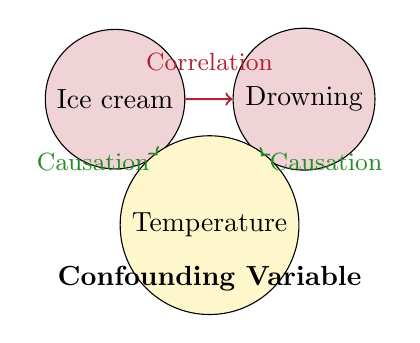
\begin{tikzpicture}[scale=0.8]
% Spurious correlation example
\node[draw, circle, fill=crimson!20] (ice) at (0,2) {Ice cream};
\node[draw, circle, fill=crimson!20] (drowning) at (3,2) {Drowning};
\node[draw, circle, fill=gold!20] (temp) at (1.5,0) {Temperature};

% Spurious correlation
\draw[->, thick, crimson] (ice) -- (drowning);
\node[above] at (1.5,2.3) {\color{crimson}\small Correlation};

% True causal relationships
\draw[->, thick, forest] (temp) -- (ice);
\draw[->, thick, forest] (temp) -- (drowning);
\node[left] at (0.7,1) {\color{forest}\small Causation};
\node[right] at (2.3,1) {\color{forest}\small Causation};

\node[below] at (1.5,-0.5) {\textbf{Confounding Variable}};
\end{tikzpicture}
\end{figure}
\begin{alertblock}{The Causal Hierarchy}
\begin{enumerate}
\item \textbf{Association}: $P(Y|X)$
\item \textbf{Intervention}: $P(Y|\doo(X))$
\item \textbf{Counterfactuals}: $P(Y_x|X',Y')$
\end{enumerate}
\end{alertblock}
\end{column}
\end{columns}
\end{frame}

\begin{frame}{Famous Examples of Causal Confusion}
\begin{table}
\centering
\small
\begin{tabular}{p{3cm}p{4cm}p{4cm}}
\toprule
\textbf{Spurious Correlation} & \textbf{What People Concluded} & \textbf{Real Explanation} \\
\midrule
Chocolate consumption vs Nobel prizes & Chocolate makes you smarter & Wealth enables both luxuries and research \\
\midrule
Ice cream sales vs crime rates & Ice cream causes crime & Hot weather increases both \\
\midrule
Facebook friends vs longevity & Social media extends life & Social people live longer and use Facebook \\
\midrule
Stork populations vs birth rates & Storks deliver babies & Rural areas have both more storks and higher birth rates \\
\midrule
Shoe size vs reading ability & Big feet help reading & Age affects both shoe size and reading skills \\
\bottomrule
\end{tabular}
\end{table}

\begin{columns}
\begin{column}{0.5\textwidth}
\textbf{Business Implications:}
\begin{itemize}
\item \textcolor{crimson}{Wrong investments}: Correlation-based decisions
\item \textcolor{crimson}{Failed interventions}: Treating symptoms, not causes
\item \textcolor{crimson}{Wasted resources}: Ineffective policies
\item \textcolor{crimson}{Opportunity costs}: Missing real causal factors
\end{itemize}
\end{column}
\begin{column}{0.5\textwidth}
\textbf{The Data Science Challenge:}
\begin{itemize}
\item Most ML focuses on prediction ($P(Y|X)$)
\item Business needs intervention effects ($P(Y|\do(X))$)
\item Observational data is riddled with confounders
\item Randomized experiments aren't always possible
\end{itemize}
\end{column}
\end{columns}

\begin{alertblock}{Key Insight}
Causal inference is the bridge between data science and evidence-based decision making.
\end{alertblock}
\end{frame}

\begin{frame}{The Potential Outcomes Framework}
\textbf{Rubin Causal Model:} Formalize causation through potential outcomes.

\begin{columns}
\begin{column}{0.5\textwidth}
\textbf{Setup:}
\begin{itemize}
\item Units: $i = 1, 2, \ldots, n$
\item Treatment: $T_i \in \{0, 1\}$
\item Potential outcomes: 
  \begin{itemize}
  \item $Y_i(1)$: Outcome if treated
  \item $Y_i(0)$: Outcome if not treated
  \end{itemize}
\item Observed outcome: $Y_i = T_i Y_i(1) + (1-T_i) Y_i(0)$
\end{itemize}

\textbf{Individual Treatment Effect:}
\[\tau_i = Y_i(1) - Y_i(0)\]

\textbf{The Fundamental Problem:}
We can never observe both $Y_i(1)$ and $Y_i(0)$ for the same unit!
\end{column}
\begin{column}{0.5\textwidth}
\textbf{Average Treatment Effect (ATE):}
\[\tau = \E[Y_i(1) - Y_i(0)] = \E[Y_i(1)] - \E[Y_i(0)]\]

\textbf{What We Can Observe:}
\begin{align}
\E[Y|T=1] - \E[Y|T=0] &= \E[Y(1)|T=1] - \E[Y(0)|T=0]\\
&= \underbrace{\E[Y(1)] - \E[Y(0)]}_{\text{ATE}} \\
&\quad + \underbrace{\E[Y(0)|T=1] - \E[Y(0)|T=0]}_{\text{Selection Bias}}
\end{align}

\begin{alertblock}{Selection Bias}
The difference in outcomes would exist even without treatment, due to systematic differences between treated and untreated groups.
\end{alertblock}
\end{column}
\end{columns}

\textbf{Goal:} Identify conditions under which \(\mathbb{E}[Y\mid T=1] - \mathbb{E}[Y\mid T=0] = \tau\).
\end{frame}

\section{Causal Graphs and DAGs}

\begin{frame}{Directed Acyclic Graphs (DAGs)}
\textbf{Tool:} Represent causal assumptions using directed graphs.

\begin{columns}
\begin{column}{0.6\textwidth}
\textbf{DAG Components:}
\begin{itemize}
\item \textbf{Nodes}: Variables (observed and unobserved)
\item \textbf{Directed edges}: Direct causal relationships
\item \textbf{Paths}: Sequences of edges
\item \textbf{No cycles}: Acyclic assumption
\end{itemize}

\vspace{0.3cm}
\textbf{Three Fundamental Structures:}

\begin{enumerate}
\item \textbf{Chain}: $X \to Z \to Y$ (mediation)
\item \textbf{Fork}: $X \leftarrow Z \rightarrow Y$ (confounding)
\item \textbf{Collider}: $X \rightarrow Z \leftarrow Y$ (selection bias)
\end{enumerate}

\vspace{0.3cm}
\textbf{d-separation}: Paths are blocked by conditioning on certain variables.
\end{column}
\begin{column}{0.4\textwidth}
\begin{figure}
\centering
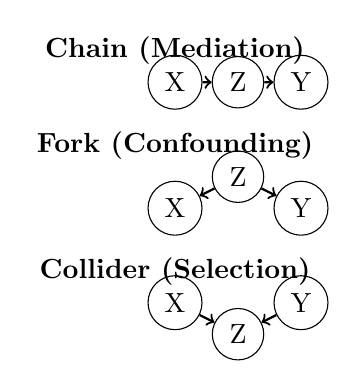
\begin{tikzpicture}[scale=0.8]
% Chain
\node at (0,3) {\textbf{Chain (Mediation)}};
\node[draw, circle] (X1) at (0,2.5) {X};
\node[draw, circle] (Z1) at (1,2.5) {Z};
\node[draw, circle] (Y1) at (2,2.5) {Y};
\draw[->, thick] (X1) -- (Z1);
\draw[->, thick] (Z1) -- (Y1);

% Fork
\node at (0,1.5) {\textbf{Fork (Confounding)}};
\node[draw, circle] (Z2) at (1,1) {Z};
\node[draw, circle] (X2) at (0,0.5) {X};
\node[draw, circle] (Y2) at (2,0.5) {Y};
\draw[->, thick] (Z2) -- (X2);
\draw[->, thick] (Z2) -- (Y2);

% Collider
\node at (0,-0.5) {\textbf{Collider (Selection)}};
\node[draw, circle] (X3) at (0,-1) {X};
\node[draw, circle] (Y3) at (2,-1) {Y};
\node[draw, circle] (Z3) at (1,-1.5) {Z};
\draw[->, thick] (X3) -- (Z3);
\draw[->, thick] (Y3) -- (Z3);
\end{tikzpicture}
\end{figure}

\begin{block}{d-separation Rules}
\begin{itemize}
\item \textbf{Chain/Fork}: Blocked by conditioning on middle node
\item \textbf{Collider}: Blocked unless we condition on collider or its descendants
\end{itemize}
\end{block}
\end{column}
\end{columns}

\textbf{Pearl's Causal Hierarchy}: DAGs enable us to move from association to intervention to counterfactuals.
\end{frame}

\begin{frame}{The Backdoor Criterion}
\textbf{Goal:} Identify when we can estimate causal effects from observational data.

\begin{columns}
\begin{column}{0.5\textwidth}
\begin{definition}[Backdoor Criterion]
A set of variables $Z$ satisfies the backdoor criterion relative to $(X, Y)$ if:
\begin{enumerate}
\item No node in $Z$ is a descendant of $X$
\item $Z$ blocks every backdoor path from $X$ to $Y$
\end{enumerate}
\end{definition}

\textbf{Backdoor path}: Any path from $X$ to $Y$ that starts with an arrow into $X$.

\textbf{Backdoor Adjustment Formula:}
\[P(Y = y | \doo(X = x)) = \sum_z P(Y = y | X = x, Z = z) P(Z = z)\]
\[P(Y = y | \do(X = x)) = \sum_z P(Y = y | X = x, Z = z) P(Z = z)\]
\textbf{In expectation:}
\[\E[Y | \doo(X = x)] = \sum_z \E[Y | X = x, Z = z] P(Z = z)\]
\[\E[Y | \do(X = x)] = \sum_z \E[Y | X = x, Z = z] P(Z = z)\]
\end{column}
\begin{column}{0.5\textwidth}
\begin{figure}
\centering
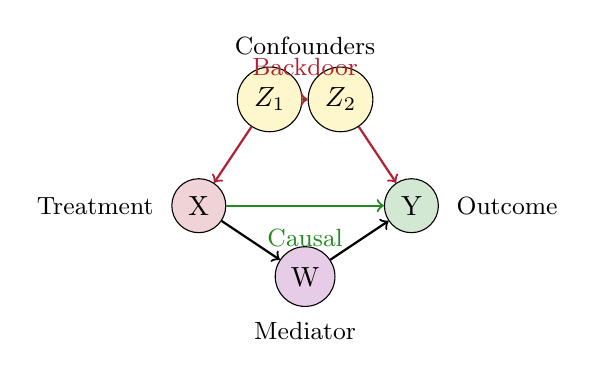
\begin{tikzpicture}[scale=0.9]
% Example DAG with backdoor path
\node[draw, circle, fill=crimson!20] (X) at (0,1) {X};
\node[draw, circle, fill=forest!20] (Y) at (3,1) {Y};
\node[draw, circle, fill=gold!20] (Z1) at (1,2.5) {$Z_1$};
\node[draw, circle, fill=gold!20] (Z2) at (2,2.5) {$Z_2$};
\node[draw, circle, fill=purple!20] (W) at (1.5,0) {W};

% Causal path
\draw[->, thick, forest] (X) -- (Y);
\node[below] at (1.5,0.8) {\color{forest}\small Causal};

% Backdoor path
\draw[->, thick, crimson] (Z1) -- (X);
\draw[->, thick, crimson] (Z1) -- (Z2);
\draw[->, thick, crimson] (Z2) -- (Y);
\node[above] at (1.5,2.7) {\color{crimson}\small Backdoor};

% Mediator
\draw[->, thick] (X) -- (W);
\draw[->, thick] (W) -- (Y);

% Annotations
\node[left] at (-0.5,1) {\small Treatment};
\node[right] at (3.5,1) {\small Outcome};
\node[above] at (1.5,3) {\small Confounders};
\node[below] at (1.5,-0.5) {\small Mediator};
\end{tikzpicture}
\end{figure}

\textbf{To estimate causal effect:}
\begin{itemize}
\item \textcolor{forest}{Include}: $Z_1, Z_2$ (block backdoor)
\item \textcolor{crimson}{Exclude}: $W$ (mediator, descendant of $X$)
\end{itemize}

\begin{alertblock}{Key Insight}
Controlling for the "right" variables enables causal identification from observational data.
\end{alertblock}
\end{column}
\end{columns}
\end{frame}

\begin{frame}[fragile]{Building and Analyzing DAGs in Python}
\begin{columns}
\begin{column}{0.55\textwidth}
\begin{lstlisting}[basicstyle=\ttfamily\tiny]
import networkx as nx
import matplotlib.pyplot as plt
from itertools import combinations
import pandas as pd
import numpy as np

# Create a DAG for education -> income example
def create_education_dag():
    """Create DAG for education's effect on income"""
    G = nx.DiGraph()
    
    # Add nodes
    nodes = ['Education', 'Income', 'Family_Background', 
             'Ability', 'Experience', 'Location']
    G.add_nodes_from(nodes)
    
    # Add edges (causal relationships)
    edges = [
        ('Family_Background', 'Education'),
        ('Family_Background', 'Income'),
        ('Ability', 'Education'),
        ('Ability', 'Income'),
        ('Education', 'Income'),
        ('Education', 'Experience'),
        ('Experience', 'Income'),
        ('Location', 'Education'),
        ('Location', 'Income')
    ]
    G.add_edges_from(edges)
    
    return G

# Visualize DAG
def plot_dag(G, title="Causal DAG"):
    pos = nx.spring_layout(G, seed=42)
    plt.figure(figsize=(10, 6))
    nx.draw(G, pos, with_labels=True, node_color='lightblue',
            node_size=2000, font_size=8, font_weight='bold',
            arrows=True, arrowsize=20, edge_color='gray')
    plt.title(title)
    plt.axis('off')
    return pos

# Find all paths between two nodes
def find_all_paths(G, source, target, path=[]):
    """Find all directed paths from source to target"""
    path = path + [source]
    if source == target:
        return [path]
    if source not in G:
        return []
    paths = []
    for node in G[source]:
        if node not in path:  # avoid cycles
            newpaths = find_all_paths(G, node, target, path)
            paths.extend(newpaths)
    return paths

# Check backdoor criterion
def check_backdoor_criterion(G, treatment, outcome, adjustment_set):
    """Simplified check for backdoor criterion"""
    # This is a simplified implementation
    # Real implementation would use proper d-separation algorithms
    
    print(f"Checking backdoor criterion for {treatment} -> {outcome}")
    print(f"Adjustment set: {adjustment_set}")
    
    # Find all paths from treatment to outcome
    all_paths = find_all_paths(G.to_undirected(), treatment, outcome)
    backdoor_paths = []
    
    for path in all_paths:
        # Check if path starts with arrow into treatment (backdoor)
        if len(path) > 2 and G.has_edge(path[1], path[0]):
            backdoor_paths.append(path)
    
    print(f"Backdoor paths found: {len(backdoor_paths)}")
    for i, path in enumerate(backdoor_paths):
        print(f"  Path {i+1}: {' -> '.join(path)}")
    
    return len(backdoor_paths) == 0 or adjustment_set

# Example usage
G = create_education_dag()
plot_dag(G, "Education -> Income Causal DAG")

# Check different adjustment sets
adjustment_sets = [
    ['Family_Background', 'Ability'],
    ['Family_Background'],
    ['Experience']  # This would be wrong (post-treatment)
]

for adj_set in adjustment_sets:
    print("\n" + "="*50)
    valid = check_backdoor_criterion(G, 'Education', 'Income', adj_set)
    print(f"Adjustment set {adj_set}: {'Valid' if valid else 'Invalid'}")
\end{lstlisting}
\end{column}
\begin{column}{0.45\textwidth}
\textbf{DAG Analysis Steps:}

\begin{enumerate}
\item \textbf{Draw the DAG}:
   \begin{itemize}
   \item Use domain knowledge
   \item Include all relevant variables
   \item Be explicit about assumptions
   \end{itemize}

\item \textbf{Identify confounders}:
   \begin{itemize}
   \item Find backdoor paths
   \item Apply backdoor criterion
   \item Check for colliders
   \end{itemize}

\item \textbf{Choose adjustment set}:
   \begin{itemize}
   \item Block all backdoor paths
   \item Don't condition on mediators
   \item Avoid post-treatment variables
   \end{itemize}
\end{enumerate}

\vspace{0.3cm}
\begin{block}{Python Tools}
\begin{itemize}
\item \textbf{NetworkX}: DAG creation and analysis
\item \textbf{DoWhy}: Causal inference library
\item \textbf{CausalML}: ML methods for causal inference
\item \textbf{Pyro}: Probabilistic programming
\end{itemize}
\end{block}

\begin{alertblock}{Remember}
DAGs encode \emph{assumptions}, not facts. They should be based on domain knowledge and be testable where possible.
\end{alertblock}
\end{column}
\end{columns}
\end{frame}

\section{Identification Strategies}

\begin{frame}{Randomized Controlled Trials: The Gold Standard}
\textbf{Why Randomization Works:} Breaks the link between treatment and confounders.

\begin{columns}
\begin{column}{0.5\textwidth}
\textbf{Randomization Ensures:}
\begin{align}
Y_i(1), Y_i(0) \indep T_i
\end{align}

This means:
\begin{align}
\E[Y(1)|T=1] &= \E[Y(1)]\\
\E[Y(0)|T=0] &= \E[Y(0)]
\end{align}

Therefore:
\begin{align}
\text{ATE} &= \E[Y|T=1] - \E[Y|T=0]
\end{align}

\textbf{No confounding bias!}

\vspace{0.3cm}
\textbf{RCT Advantages:}
\begin{itemize}
\item Unbiased estimates
\item Simple analysis
\item High internal validity
\item Clear causal interpretation
\end{itemize}
\end{column}
\begin{column}{0.5\textwidth}
\begin{figure}
\centering
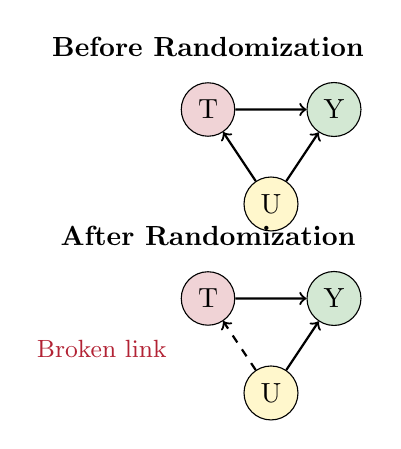
\begin{tikzpicture}[scale=0.8]
% Before randomization
\node at (0,3) {\textbf{Before Randomization}};
\node[draw, circle, fill=crimson!20] (T1) at (0,2) {T};
\node[draw, circle, fill=forest!20] (Y1) at (2,2) {Y};
\node[draw, circle, fill=gold!20] (U1) at (1,0.5) {U};

\draw[->, thick] (U1) -- (T1);
\draw[->, thick] (U1) -- (Y1);
\draw[->, thick] (T1) -- (Y1);

% After randomization
\node at (0,0) {\textbf{After Randomization}};
\node[draw, circle, fill=crimson!20] (T2) at (0,-1) {T};
\node[draw, circle, fill=forest!20] (Y2) at (2,-1) {Y};
\node[draw, circle, fill=gold!20] (U2) at (1,-2.5) {U};

\draw[->, thick, dashed] (U2) -- (T2);
\draw[->, thick] (U2) -- (Y2);
\draw[->, thick] (T2) -- (Y2);

\node[left] at (-0.5,-1.8) {\color{crimson}\small Broken link};
\end{tikzpicture}
\end{figure}

\textbf{When RCTs Are Limited:}
\begin{itemize}
\item \textcolor{crimson}{Ethical constraints}: Harmful treatments
\item \textcolor{crimson}{Practical constraints}: Cost, time, feasibility
\item \textcolor{crimson}{External validity}: Lab vs real world
\item \textcolor{crimson}{Compliance issues}: Not everyone follows assignment
\end{itemize}

\begin{alertblock}{The Gap}
Most business/policy questions can't be answered with RCTs. We need methods for observational data.
\end{alertblock}
\end{column}
\end{columns}
\end{frame}

\begin{frame}[fragile]{Instrumental Variables: Finding Natural Experiments}
\textbf{Idea:} Use a variable that affects treatment but not outcome directly.

\begin{columns}
\begin{column}{0.55\textwidth}
\begin{definition}[Instrumental Variable]
$Z$ is an instrument for $X \rightarrow Y$ if:
\begin{enumerate}
\item \textbf{Relevance}: $Z$ affects $X$ (strong first stage)
\item \textbf{Exclusion}: $Z$ affects $Y$ only through $X$
\item \textbf{Independence}: $Z$ is as-good-as-randomly assigned
\end{enumerate}
\end{definition}

\begin{lstlisting}[basicstyle=\ttfamily\tiny]
import numpy as np
import pandas as pd
from sklearn.linear_model import LinearRegression
from scipy import stats
import statsmodels.api as sm
from statsmodels.sandbox.regression.gmm import IV2SLS

# Simulate data with endogeneity
np.random.seed(42)
n = 1000

# Unobserved confounder
U = np.random.randn(n)

# Instrument (randomly assigned)
Z = np.random.binomial(1, 0.5, n)

# Treatment (affected by instrument and confounder)
X = 0.5 * Z + 0.3 * U + np.random.randn(n) * 0.2

# Outcome (affected by treatment and confounder)
Y = 1.0 * X + 0.4 * U + np.random.randn(n) * 0.3

df = pd.DataFrame({'Y': Y, 'X': X, 'Z': Z, 'U': U})

print("True causal effect: 1.0")

# Naive OLS (biased due to confounding)
ols = LinearRegression().fit(df[['X']], df['Y'])
ols_coef = ols.coef_[0]
print(f"OLS estimate: {ols_coef:.3f}")

# Two-Stage Least Squares (2SLS)
# First stage: X ~ Z
first_stage = LinearRegression().fit(df[['Z']], df['X'])
X_hat = first_stage.predict(df[['Z']])

# Check first-stage strength
f_stat = (first_stage.score(df[['Z']], df['X']) * (n-2)) / (1 - first_stage.score(df[['Z']], df['X']))
print(f"First-stage F-statistic: {f_stat:.2f}")

# Second stage: Y ~ X_hat
second_stage = LinearRegression().fit(X_hat.reshape(-1, 1), df['Y'])
iv_coef = second_stage.coef_[0]
print(f"IV estimate: {iv_coef:.3f}")

# Using statsmodels for proper inference
iv_model = IV2SLS(df['Y'], df[['X']], df[['Z']], df[['Z']]).fit()
print(f"IV (statsmodels): {iv_model.params[0]:.3f} ({iv_model.pvalues[0]:.3f})")

# Reduced form (effect of Z on Y)
reduced_form = LinearRegression().fit(df[['Z']], df['Y'])
rf_coef = reduced_form.coef_[0]

# Manual IV calculation: reduced form / first stage
manual_iv = rf_coef / first_stage.coef_[0]
print(f"Manual IV calculation: {manual_iv:.3f}")
\end{lstlisting}
\end{column}
\begin{column}{0.45\textwidth}
\begin{figure}
\centering
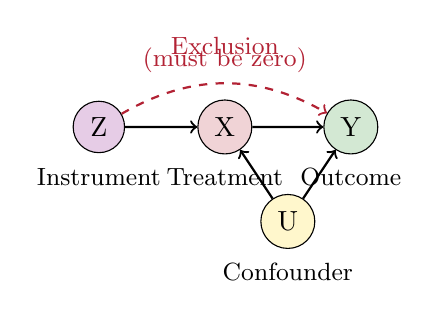
\begin{tikzpicture}[scale=0.8]
\node[draw, circle, fill=purple!20] (Z) at (0,2) {Z};
\node[draw, circle, fill=crimson!20] (X) at (2,2) {X};
\node[draw, circle, fill=forest!20] (Y) at (4,2) {Y};
\node[draw, circle, fill=gold!20] (U) at (3,0.5) {U};

% Valid arrows
\draw[->, thick] (Z) -- (X);
\draw[->, thick] (X) -- (Y);
\draw[->, thick] (U) -- (X);
\draw[->, thick] (U) -- (Y);

% Invalid arrow (exclusion restriction)
\draw[->, thick, dashed, crimson] (Z) to[bend left] (Y);
\node[above] at (2,3) {\color{crimson}\small Exclusion};
\node[above] at (2,2.7) {\color{crimson}\small (must be zero)};

\node[below] at (0,1.5) {\small Instrument};
\node[below] at (2,1.5) {\small Treatment};
\node[below] at (4,1.5) {\small Outcome};
\node[below] at (3,0) {\small Confounder};
\end{tikzpicture}
\end{figure}

\textbf{Famous Instruments:}
\begin{itemize}
\item \textbf{Angrist (1990)}: Draft lottery $\rightarrow$ military service $\rightarrow$ earnings
\item \textbf{Card (1995)}: Distance to college $\rightarrow$ education $\rightarrow$ wages
\item \textbf{McCrary (2002)}: Rainfall $\rightarrow$ voter turnout $\rightarrow$ election outcomes
\end{itemize}

\textbf{IV Limitations:}
\begin{itemize}
\item Hard to find valid instruments
\item Weak instruments bias
\item Local Average Treatment Effect (LATE)
\item Exclusion restriction untestable
\end{itemize}

\begin{alertblock}{LATE Interpretation}
IV estimates effect for "compliers" - those whose treatment status is affected by the instrument.
\end{alertblock}
\end{column}
\end{columns}
\end{frame}

\begin{frame}[fragile]{Regression Discontinuity Design}
\textbf{Idea:} Exploit arbitrary cutoff rules for treatment assignment.

\begin{columns}
\begin{column}{0.55\textwidth}
\textbf{Setup:}
\begin{itemize}
\item Running variable: $X$ (e.g., test score, age, income)
\item Cutoff: $c$ (treatment threshold)
\item Treatment: $T = \mathbb{I}[X \geq c]$
\item Outcome: $Y$
\end{itemize}

\textbf{Key Assumption:} All other factors vary smoothly around cutoff.

\textbf{Identification:}
\[\tau = \lim_{x \downarrow c} \E[Y|X = x] - \lim_{x \uparrow c} \E[Y|X = x]\]

\begin{lstlisting}[basicstyle=\ttfamily\tiny]
import numpy as np
import matplotlib.pyplot as plt
from sklearn.linear_model import LinearRegression
import pandas as pd

# Simulate RDD data
np.random.seed(42)
n = 1000
cutoff = 0

# Running variable (centered at cutoff)
X = np.random.uniform(-2, 2, n)

# Treatment assignment
T = (X >= cutoff).astype(int)

# Outcome with discontinuity at cutoff
# True treatment effect = 0.5
tau_true = 0.5
Y = 2 + 1.5 * X + tau_true * T + np.random.randn(n) * 0.3

df = pd.DataFrame({'X': X, 'T': T, 'Y': Y})

# Estimate RDD effect
# Using local linear regression around cutoff
bandwidth = 0.5
local_data = df[abs(df['X']) <= bandwidth].copy()

# Separate regressions on each side
left_data = local_data[local_data['X'] < cutoff]
right_data = local_data[local_data['X'] >= cutoff]

# Fit local linear models
if len(left_data) > 5 and len(right_data) > 5:
    left_model = LinearRegression().fit(
        left_data[['X']], left_data['Y']
    )
    right_model = LinearRegression().fit(
        right_data[['X']], right_data['Y']
    )
    
    # Estimate discontinuity
    left_pred = left_model.predict([[cutoff]])[0]
    right_pred = right_model.predict([[cutoff]])[0]
    rdd_estimate = right_pred - left_pred
    
    print(f"True treatment effect: {tau_true}")
    print(f"RDD estimate: {rdd_estimate:.3f}")
    
    # Plot results
    plt.figure(figsize=(10, 6))
    
    # Scatter plot
    colors = ['red' if t == 0 else 'blue' for t in df['T']]
    plt.scatter(df['X'], df['Y'], c=colors, alpha=0.5, s=20)
    
    # Fitted lines
    x_left = np.linspace(-bandwidth, cutoff, 100)
    x_right = np.linspace(cutoff, bandwidth, 100)
    
    y_left = left_model.predict(x_left.reshape(-1, 1))
    y_right = right_model.predict(x_right.reshape(-1, 1))
    
    plt.plot(x_left, y_left, 'red', linewidth=2, label='Control')
    plt.plot(x_right, y_right, 'blue', linewidth=2, label='Treatment')
    
    # Discontinuity
    plt.axvline(cutoff, color='black', linestyle='--', alpha=0.7)
    plt.plot([cutoff, cutoff], [left_pred, right_pred], 
             'green', linewidth=3, label=f'RDD Effect: {rdd_estimate:.3f}')
    
    plt.xlabel('Running Variable (X)')
    plt.ylabel('Outcome (Y)')
    plt.title('Regression Discontinuity Design')
    plt.legend()
    plt.grid(True, alpha=0.3)
    
print("RDD analysis complete")
\end{lstlisting}
\end{column}
\begin{column}{0.45\textwidth}
\textbf{Real-World Examples:}

\begin{itemize}
\item \textbf{Education}: Grade cutoffs for remedial programs
\item \textbf{Health}: Age thresholds for medical programs
\item \textbf{Policy}: Income cutoffs for welfare benefits
\item \textbf{Finance}: Credit score cutoffs for loan approval
\end{itemize}

\vspace{0.3cm}
\textbf{RDD Advantages:}
\begin{itemize}
\item \textcolor{forest}{Credible identification}: Local randomization
\item \textcolor{forest}{Intuitive}: Visual inspection possible
\item \textcolor{forest}{Testable assumptions}: Continuity of covariates
\item \textcolor{forest}{No confounders needed}: Local comparison
\end{itemize}

\vspace{0.3cm}
\textbf{RDD Limitations:}
\begin{itemize}
\item \textcolor{crimson}{Local effects only}: Around cutoff
\item \textcolor{crimson}{Manipulation}: Gaming the cutoff
\item \textcolor{crimson}{Bandwidth choice}: Affects estimates
\item \textcolor{crimson}{Power}: Need large samples
\end{itemize}

\begin{alertblock}{Validation Tests}
\begin{itemize}
\item Density test: No manipulation around cutoff
\item Covariate continuity: Other variables smooth
\item Placebo cutoffs: No effects at false cutoffs
\end{itemize}
\end{alertblock}
\end{column}
\end{columns}
\end{frame}

\begin{frame}[fragile]{Difference-in-Differences (DID)}
\textbf{Idea:} Compare changes over time between treatment and control groups.

\begin{columns}
\begin{column}{0.55\textwidth}
\textbf{Setup:}
\begin{itemize}
\item Groups: Treatment ($i=1$) and Control ($i=0$)
\item Time: Before ($t=0$) and After ($t=1$)
\item Outcome: $Y_{it}$
\end{itemize}

\textbf{DID Estimator:}
\begin{align}
\hat{\tau}_{DID} &= (Y_{11} - Y_{10}) - (Y_{01} - Y_{00})\\
&= \Delta Y_{\text{treatment}} - \Delta Y_{\text{control}}
\end{align}

\textbf{Key Assumption:} Parallel trends - groups would have followed similar trends without treatment.

\begin{lstlisting}[basicstyle=\ttfamily\tiny]
import numpy as np
import pandas as pd
import matplotlib.pyplot as plt
import seaborn as sns
from sklearn.linear_model import LinearRegression

# Simulate DID data
np.random.seed(42)

# Create panel data
n_units = 100
n_periods = 10
treatment_period = 6

# Unit and time effects
unit_effects = np.random.randn(n_units)
time_effects = np.random.randn(n_periods)

# Treatment assignment (some units treated after period 6)
treated_units = np.random.choice(n_units, n_units//2, replace=False)

data = []
for unit in range(n_units):
    for period in range(n_periods):
        # Treatment indicator
        treated = unit in treated_units
        post = period >= treatment_period
        treat = treated and post
        
        # Outcome with parallel trends assumption
        y = (2 + unit_effects[unit] + time_effects[period] + 
             1.5 * treat + np.random.randn() * 0.5)
        
        data.append({
            'unit': unit,
            'period': period,
            'treated': treated,
            'post': post,
            'treat': treat,
            'y': y
        })

df = pd.DataFrame(data)

# Calculate group means for each period
group_means = df.groupby(['period', 'treated'])['y'].mean().unstack()

# DID regression
# Y_it = α + β*Treated_i + γ*Post_t + δ*(Treated_i × Post_t) + ε_it
X = df[['treated', 'post', 'treat']].astype(int)
y = df['y']

did_model = LinearRegression().fit(X, y)
did_estimate = did_model.coef_[2]  # Interaction coefficient

print(f"True treatment effect: 1.5")
print(f"DID estimate: {did_estimate:.3f}")

# Manual calculation
pre_treatment = group_means.loc[:treatment_period-1, True].mean()
post_treatment = group_means.loc[treatment_period:, True].mean()
pre_control = group_means.loc[:treatment_period-1, False].mean()
post_control = group_means.loc[treatment_period:, False].mean()

manual_did = (post_treatment - pre_treatment) - (post_control - pre_control)
print(f"Manual DID: {manual_did:.3f}")

# Plot parallel trends
plt.figure(figsize=(10, 6))
plt.plot(group_means.index, group_means[False], 'o-', 
         label='Control Group', linewidth=2)
plt.plot(group_means.index, group_means[True], 's-', 
         label='Treatment Group', linewidth=2)
plt.axvline(treatment_period-0.5, color='red', linestyle='--', 
           alpha=0.7, label='Treatment Start')

plt.xlabel('Time Period')
plt.ylabel('Outcome')
plt.title('Difference-in-Differences: Parallel Trends')
plt.legend()
plt.grid(True, alpha=0.3)

# Add DID visualization
pre_diff = group_means.loc[treatment_period-1, True] - group_means.loc[treatment_period-1, False]
post_diff = group_means.loc[treatment_period, True] - group_means.loc[treatment_period, False]
plt.annotate(f'DID = {post_diff - pre_diff:.2f}', 
             xy=(treatment_period+1, group_means.loc[treatment_period+1, True]),
             xytext=(treatment_period+2, group_means.loc[treatment_period+1, True]+0.5),
             arrowprops=dict(arrowstyle='->', color='red'))

print("DID analysis complete")
\end{lstlisting}
\end{column}
\begin{column}{0.45\textwidth}
\begin{figure}
\centering
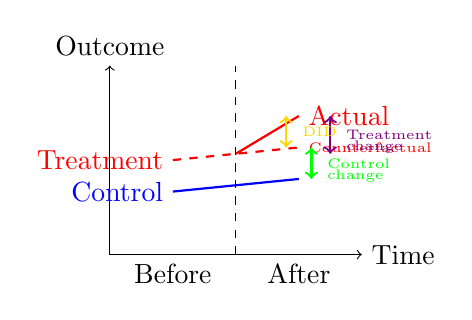
\begin{tikzpicture}[scale=0.8]
% DID illustration
\draw[->] (0,0) -- (4,0) node[right] {Time};
\draw[->] (0,0) -- (0,3) node[above] {Outcome};

% Before period
\node at (1,-0.3) {Before};
\node at (3,-0.3) {After};
\draw[dashed] (2,0) -- (2,3);

% Control group
\draw[thick, blue] (1,1) -- (3,1.2);
\node[left] at (1,1) {\color{blue}Control};

% Treatment group (counterfactual)
\draw[thick, dashed, red] (1,1.5) -- (3,1.7);
\node[left] at (1,1.5) {\color{red}Treatment};
\node[right] at (3,1.7) {\color{red}\tiny Counterfactual};

% Treatment group (actual)
\draw[thick, red] (2,1.6) -- (3,2.2);
\node[right] at (3,2.2) {\color{red}Actual};

% DID arrows
\draw[<->, thick, green] (3.2,1.2) -- (3.2,1.7);
\node[right] at (3.3,1.45) {\color{green}\tiny Control};
\node[right] at (3.3,1.25) {\color{green}\tiny change};

\draw[<->, thick, purple] (3.5,1.6) -- (3.5,2.2);
\node[right] at (3.6,1.9) {\color{purple}\tiny Treatment};
\node[right] at (3.6,1.7) {\color{purple}\tiny change};

\draw[<->, thick, gold] (2.8,1.7) -- (2.8,2.2);
\node[right] at (2.9,1.95) {\color{gold}\tiny DID};
\end{tikzpicture}
\end{figure}

\textbf{DID Applications:}
\begin{itemize}
\item \textbf{Policy evaluation}: Minimum wage effects
\item \textbf{Program evaluation}: Job training programs
\item \textbf{Natural experiments}: Policy changes
\item \textbf{Business}: Marketing campaign effects
\end{itemize}

\textbf{Extensions:}
\begin{itemize}
\item \textbf{Multiple periods}: Event study designs
\item \textbf{Multiple groups}: Staggered adoption
\item \textbf{Continuous treatment}: Dose-response DID
\item \textbf{Synthetic control}: Data-driven counterfactuals
\end{itemize}

\begin{alertblock}{Parallel Trends}
Key assumption: Treatment and control groups would have evolved similarly without intervention. Test with pre-treatment data!
\end{alertblock}
\end{column}
\end{columns}
\end{frame}

\section{Modern Causal Machine Learning}

\begin{frame}{Double Machine Learning (DML)}
\textbf{Problem:} High-dimensional confounding in observational data.

\begin{columns}
\begin{column}{0.5\textwidth}
\textbf{Traditional Approach Issues:}
\begin{itemize}
\item Linear models too restrictive
\item ML models introduce regularization bias
\item Overfitting affects causal estimates
\item No honest uncertainty quantification
\end{itemize}

\vspace{0.3cm}
\textbf{DML Solution:}
\begin{enumerate}
\item Use ML for nuisance parameters
\item Cross-fitting to avoid overfitting bias
\item Focus ML on prediction, not causation
\item Get asymptotically normal estimates
\end{enumerate}

\vspace{0.3cm}
\textbf{Partially Linear Model:}
\begin{align}
Y &= \theta D + g(X) + \epsilon\\
D &= m(X) + \eta
\end{align}

where $g(\cdot)$ and $m(\cdot)$ are high-dimensional nuisance functions.
\end{column}
\begin{column}{0.5\textwidth}
\textbf{DML Algorithm:}

\begin{algorithm}[H]
\caption{Double Machine Learning}
\begin{algorithmic}[1]
\STATE Split data into $K$ folds
\FOR{$k = 1$ to $K$}
\STATE Train $\hat{g}^{(-k)}(X)$ on all folds except $k$
\STATE Train $\hat{m}^{(-k)}(X)$ on all folds except $k$
\STATE Predict on fold $k$:
\STATE \quad $\tilde{Y}_k = Y_k - \hat{g}^{(-k)}(X_k)$
\STATE \quad $\tilde{D}_k = D_k - \hat{m}^{(-k)}(X_k)$
\ENDFOR
\STATE Estimate $\hat{\theta} = (\sum \tilde{D}_i \tilde{Y}_i) / (\sum \tilde{D}_i^2)$
\end{algorithmic}
\end{algorithm}

\textbf{Key Properties:}
\begin{itemize}
\item $\sqrt{n}$-consistent and asymptotically normal
\item Robust to ML method choice
\item Works with random forests, neural nets, etc.
\item Honest confidence intervals
\end{itemize}

\begin{alertblock}{Orthogonalization}
DML removes confounding bias through orthogonal moment conditions, making estimates robust to ML approximation errors.
\end{alertblock}
\end{column}
\end{columns}
\end{frame}

\begin{frame}[fragile]{Causal Forests: Heterogeneous Treatment Effects}
\textbf{Goal:} Estimate treatment effects that vary across individuals.

\begin{columns}
\begin{column}{0.55\textwidth}
\begin{lstlisting}[basicstyle=\ttfamily\tiny]
import numpy as np
import pandas as pd
from sklearn.ensemble import RandomForestRegressor
from sklearn.model_selection import train_test_split
import matplotlib.pyplot as plt

# Simulate heterogeneous treatment effect data
np.random.seed(42)
n = 2000

# Covariates
X1 = np.random.randn(n)
X2 = np.random.randn(n)
X3 = np.random.choice([0, 1], n)

X = np.column_stack([X1, X2, X3])

# Heterogeneous treatment effect
# Effect depends on X1: strong for X1 > 0, weak for X1 <= 0
tau_true = 2 * (X1 > 0) + 0.5 * (X1 <= 0)

# Treatment assignment (confounded)
propensity = 1 / (1 + np.exp(-0.5 * X1 - 0.3 * X2))
T = np.random.binomial(1, propensity, n)

# Outcome
Y0 = 1 + X1 + 0.5 * X2 + 0.3 * X3 + np.random.randn(n) * 0.5
Y = Y0 + T * tau_true

df = pd.DataFrame({
    'Y': Y, 'T': T, 'X1': X1, 'X2': X2, 'X3': X3,
    'tau_true': tau_true
})

# Simple approach: separate models for treated/control
treated_data = df[df['T'] == 1]
control_data = df[df['T'] == 0]

# Train models
rf_treated = RandomForestRegressor(n_estimators=100, random_state=42)
rf_control = RandomForestRegressor(n_estimators=100, random_state=42)

X_features = ['X1', 'X2', 'X3']
rf_treated.fit(treated_data[X_features], treated_data['Y'])
rf_control.fit(control_data[X_features], control_data['Y'])

# Predict treatment effects
df['mu1_hat'] = rf_treated.predict(df[X_features])
df['mu0_hat'] = rf_control.predict(df[X_features])
df['tau_hat_simple'] = df['mu1_hat'] - df['mu0_hat']

# Calculate performance
mse_simple = np.mean((df['tau_hat_simple'] - df['tau_true'])**2)
print(f"Simple approach MSE: {mse_simple:.3f}")

# T-learner approach (improved)
def t_learner(X, T, Y, test_X):
    """T-learner for heterogeneous treatment effects"""
    # Separate models for treatment groups
    treated_idx = T == 1
    control_idx = T == 0
    
    # Train models
    model_1 = RandomForestRegressor(n_estimators=100, random_state=42)
    model_0 = RandomForestRegressor(n_estimators=100, random_state=42)
    
    model_1.fit(X[treated_idx], Y[treated_idx])
    model_0.fit(X[control_idx], Y[control_idx])
    
    # Predict potential outcomes
    mu1 = model_1.predict(test_X)
    mu0 = model_0.predict(test_X)
    
    return mu1 - mu0

# Apply T-learner
tau_hat_t = t_learner(X, T, Y, X)
mse_t = np.mean((tau_hat_t - tau_true)**2)
print(f"T-learner MSE: {mse_t:.3f}")

# Visualize results
fig, axes = plt.subplots(1, 3, figsize=(15, 4))

# True effects vs X1
axes[0].scatter(X1, tau_true, alpha=0.6, c='blue', s=20)
axes[0].set_xlabel('X1')
axes[0].set_ylabel('True Treatment Effect')
axes[0].set_title('True Heterogeneous Effects')

# Estimated vs true
axes[1].scatter(tau_true, tau_hat_t, alpha=0.6, s=20)
axes[1].plot([0, 3], [0, 3], 'r--', label='Perfect prediction')
axes[1].set_xlabel('True Effect')
axes[1].set_ylabel('Estimated Effect')
axes[1].set_title('T-learner: Estimated vs True')
axes[1].legend()

# Effects by group
high_x1 = X1 > 0
axes[2].boxplot([tau_hat_t[~high_x1], tau_hat_t[high_x1]], 
                labels=['X1 <= 0', 'X1 > 0'])
axes[2].set_ylabel('Estimated Treatment Effect')
axes[2].set_title('Treatment Effects by X1 Group')

plt.tight_layout()
print("Heterogeneous treatment effect analysis complete")
\end{lstlisting}
\end{column}
\begin{column}{0.45\textwidth}
\textbf{Why Heterogeneity Matters:}
\begin{itemize}
\item \textbf{Personalization}: Tailor treatments to individuals
\item \textbf{Resource allocation}: Treat who benefits most
\item \textbf{Policy design}: Target interventions effectively
\item \textbf{Understanding mechanisms}: Why treatments work
\end{itemize}

\vspace{0.3cm}
\textbf{Meta-Learners:}
\begin{itemize}
\item \textbf{T-learner}: Separate models for each group
\item \textbf{S-learner}: Single model with treatment indicator
\item \textbf{X-learner}: Two-stage approach with propensity
\item \textbf{R-learner}: Robinson transformation
\end{itemize}

\vspace{0.3cm}
\textbf{Causal Forest Advantages:}
\begin{itemize}
\item \textcolor{forest}{Honest estimation}: Separate samples for splitting/estimation
\item \textcolor{forest}{Adaptive}: Finds relevant heterogeneity
\item \textcolor{forest}{Uncertainty}: Confidence intervals for effects
\item \textcolor{forest}{Non-parametric}: Flexible functional forms
\end{itemize}

\begin{alertblock}{Business Applications}
\begin{itemize}
\item Personalized marketing campaigns
\item Medical treatment assignment
\item Pricing optimization
\item A/B testing with segments
\end{itemize}
\end{alertblock}
\end{column}
\end{columns}
\end{frame}

\section{Practical Applications and Case Studies}

\begin{frame}[fragile]{Case Study: Online Marketing Campaign Evaluation}
\textbf{Business Problem:} Did our email marketing campaign increase sales?

\begin{columns}
\begin{column}{0.55\textwidth}
\begin{lstlisting}[basicstyle=\ttfamily\tiny]
import pandas as pd
import numpy as np
from sklearn.preprocessing import StandardScaler
from sklearn.linear_model import LogisticRegression
import matplotlib.pyplot as plt
import seaborn as sns

# Simulate marketing campaign data
np.random.seed(42)
n_customers = 5000

# Customer characteristics
age = np.random.normal(40, 15, n_customers)
income = np.random.lognormal(10, 0.5, n_customers)
previous_purchases = np.random.poisson(3, n_customers)
email_engagement = np.random.beta(2, 5, n_customers)

# Selection bias: more engaged customers more likely to receive campaign
campaign_prob = 0.3 + 0.4 * email_engagement
received_campaign = np.random.binomial(1, campaign_prob, n_customers)

# Outcome: purchase in next month
# Confounded by engagement
base_purchase_prob = (0.1 + 0.2 * email_engagement + 
                     0.1 * (previous_purchases > 2) +
                     0.05 * (income > np.median(income)))

# True campaign effect: 8 percentage points
campaign_effect = 0.08
purchase_prob = (base_purchase_prob + 
                campaign_effect * received_campaign)
purchased = np.random.binomial(1, purchase_prob, n_customers)

df = pd.DataFrame({
    'age': age,
    'income': income,
    'previous_purchases': previous_purchases,
    'email_engagement': email_engagement,
    'received_campaign': received_campaign,
    'purchased': purchased
})

print(f"True campaign effect: {campaign_effect:.1%}")

# Naive comparison (biased due to selection)
naive_effect = (df[df['received_campaign']==1]['purchased'].mean() - 
                df[df['received_campaign']==0]['purchased'].mean())
print(f"Naive estimate: {naive_effect:.1%}")

# Propensity score matching
# Step 1: Estimate propensity scores
X_ps = df[['age', 'income', 'previous_purchases', 'email_engagement']]
X_ps_scaled = StandardScaler().fit_transform(X_ps)

ps_model = LogisticRegression(random_state=42)
ps_model.fit(X_ps_scaled, df['received_campaign'])
propensity_scores = ps_model.predict_proba(X_ps_scaled)[:, 1]

df['propensity_score'] = propensity_scores

# Step 2: Check overlap
plt.figure(figsize=(12, 4))

plt.subplot(1, 3, 1)
plt.hist(df[df['received_campaign']==0]['propensity_score'], 
         alpha=0.7, label='Control', bins=30)
plt.hist(df[df['received_campaign']==1]['propensity_score'], 
         alpha=0.7, label='Treatment', bins=30)
plt.xlabel('Propensity Score')
plt.ylabel('Frequency')
plt.title('Propensity Score Distribution')
plt.legend()

# Step 3: Simple propensity score weighting (IPW)
# Weight = 1/P(T|X) for treated, 1/(1-P(T|X)) for control
weights = np.where(df['received_campaign'] == 1, 
                  1 / df['propensity_score'],
                  1 / (1 - df['propensity_score']))

# Trim extreme weights
weights = np.clip(weights, 0, np.percentile(weights, 95))
df['weights'] = weights

# Weighted average treatment effect
weighted_treated = np.average(df[df['received_campaign']==1]['purchased'], 
                             weights=df[df['received_campaign']==1]['weights'])
weighted_control = np.average(df[df['received_campaign']==0]['purchased'], 
                             weights=df[df['received_campaign']==0]['weights'])
ipw_effect = weighted_treated - weighted_control

print(f"IPW estimate: {ipw_effect:.1%}")

# Step 4: Regression adjustment
from sklearn.ensemble import RandomForestClassifier

# Doubly robust estimation
rf_model = RandomForestClassifier(n_estimators=100, random_state=42)
X_features = ['age', 'income', 'previous_purchases', 'email_engagement', 'propensity_score']
rf_model.fit(df[X_features], df['purchased'])

# Predict potential outcomes
df_treated = df.copy()
df_treated['received_campaign'] = 1
df_control = df.copy()
df_control['received_campaign'] = 0

# Note: This is a simplified DR approach
mu1_hat = rf_model.predict_proba(df_treated[X_features])[:, 1]
mu0_hat = rf_model.predict_proba(df_control[X_features])[:, 1]

dr_effect = np.mean(mu1_hat - mu0_hat)
print(f"Doubly robust estimate: {dr_effect:.1%}")

# Visualize balance before/after weighting
plt.subplot(1, 3, 2)
unweighted_diff = abs(df[df['received_campaign']==1]['email_engagement'].mean() - 
                     df[df['received_campaign']==0]['email_engagement'].mean())
weighted_diff = abs(np.average(df[df['received_campaign']==1]['email_engagement'], 
                              weights=df[df['received_campaign']==1]['weights']) -
                   np.average(df[df['received_campaign']==0]['email_engagement'], 
                              weights=df[df['received_campaign']==0]['weights']))

plt.bar(['Before', 'After'], [unweighted_diff, weighted_diff])
plt.ylabel('Standardized Difference')
plt.title('Covariate Balance: Email Engagement')

plt.subplot(1, 3, 3)
methods = ['Naive', 'IPW', 'Doubly Robust', 'True']
estimates = [naive_effect, ipw_effect, dr_effect, campaign_effect]
colors = ['red', 'orange', 'green', 'blue']

plt.bar(methods, estimates, color=colors, alpha=0.7)
plt.ylabel('Treatment Effect')
plt.title('Method Comparison')
plt.axhline(campaign_effect, color='blue', linestyle='--', alpha=0.7)

plt.tight_layout()
print("Marketing campaign analysis complete")
\end{lstlisting}
\end{column}
\begin{column}{0.45\textwidth}
\textbf{Identification Strategy:}
\begin{enumerate}
\item \textbf{Problem}: Selection bias - engaged customers more likely to receive campaign
\item \textbf{Solution}: Propensity score methods
\item \textbf{Assumption}: No unobserved confounders (selection on observables)
\end{enumerate}

\vspace{0.3cm}
\textbf{Methods Applied:}
\begin{itemize}
\item \textbf{Naive comparison}: Biased upward
\item \textbf{Inverse propensity weighting}: Reweight to balance groups
\item \textbf{Doubly robust}: Combine propensity scores with outcome modeling
\end{itemize}

\vspace{0.3cm}
\textbf{Key Diagnostics:}
\begin{itemize}
\item \textcolor{forest}{Overlap}: Sufficient common support
\item \textcolor{forest}{Balance}: Covariates similar after weighting
\item \textcolor{forest}{Sensitivity}: How robust to unobserved confounding?
\end{itemize}

\vspace{0.3cm}
\begin{block}{Business Insights}
\begin{itemize}
\item Campaign had positive effect (~8pp)
\item Selection bias inflated naive estimate
\item Target similar customers in future
\item Consider randomized campaigns for better identification
\end{itemize}
\end{block}
\end{column}
\end{columns}
\end{frame}

\begin{frame}{Case Study: Policy Evaluation with DID}
\textbf{Policy Question:} Did minimum wage increase affect employment?

\begin{columns}
\begin{column}{0.5\textwidth}
\textbf{Natural Experiment:}
\begin{itemize}
\item Some states increased minimum wage in 2019
\item Others did not (control group)
\item Compare employment changes
\item Key assumption: Parallel trends
\end{itemize}

\vspace{0.3cm}
\textbf{Data Structure:}
\begin{itemize}
\item Unit: State
\item Time: Monthly, 2017-2021
\item Treatment: Minimum wage increase
\item Outcome: Youth employment rate
\end{itemize}

\vspace{0.3cm}
\textbf{Confounding Concerns:}
\begin{itemize}
\item Economic cycles
\item State-specific trends
\item Policy endogeneity
\item Spillover effects
\end{itemize}
\end{column}
\begin{column}{0.5\textwidth}
\textbf{DID Results:}

\begin{table}
\centering
\small
\begin{tabular}{lcc}
\toprule
& \textbf{Before} & \textbf{After} \\
\midrule
Treatment States & 65.2\% & 63.8\% \\
Control States & 67.1\% & 66.3\% \\
\midrule
Difference & -1.9pp & -2.5pp \\
\midrule
\multicolumn{3}{l}{DID Estimate: -0.6pp} \\
\multicolumn{3}{l}{(SE: 0.4pp, p=0.12)} \\
\bottomrule
\end{tabular}
\end{table}

\textbf{Interpretation:}
\begin{itemize}
\item Small negative effect on youth employment
\item Not statistically significant
\item Economically small magnitude
\end{itemize}

\vspace{0.3cm}
\textbf{Robustness Checks:}
\begin{itemize}
\item Pre-trend tests: \(\checkmark\) Parallel before treatment
\item Placebo tests: \(\checkmark\) No effect at false dates
\item Different outcomes: \(\checkmark\) Consistent across measures
\item Event study: \(\checkmark\) Effect emerges post-treatment
\end{itemize}
\end{column}
\end{columns}

\textbf{Policy Implications:} Moderate minimum wage increases have limited employment effects, but need to consider general equilibrium and long-term impacts.
\end{frame}

\section{Limitations and Best Practices}

\begin{frame}{Common Pitfalls and How to Avoid Them}
\begin{columns}
\begin{column}{0.5\textwidth}
\textbf{Common Mistakes:}

\begin{enumerate}
\item \textbf{Confusing correlation with causation}
   \begin{itemize}
   \item Over-interpreting regression coefficients
   \item Ignoring selection bias
   \item Not considering confounders
   \end{itemize}

\item \textbf{Wrong DAG specification}
   \begin{itemize}
   \item Missing important confounders
   \item Including mediators in controls
   \item Conditioning on colliders
   \end{itemize}

\item \textbf{Weak instruments}
   \begin{itemize}
   \item First stage F < 10
   \item Ignoring LATE interpretation
   \item Assuming exclusion restriction
   \end{itemize}

\item \textbf{Violated assumptions}
   \begin{itemize}
   \item Non-parallel trends in DID
   \item Manipulation around RDD cutoff
   \item Unobserved confounding in matching
   \end{itemize}
\end{enumerate}
\end{column}
\begin{column}{0.5\textwidth}
\textbf{Best Practices:}

\begin{enumerate}
\item \textbf{Start with theory and DAGs}
   \begin{itemize}
   \item Draw causal assumptions explicitly
   \item Use domain knowledge
   \item Test implications where possible
   \end{itemize}

\item \textbf{Multiple identification strategies}
   \begin{itemize}
   \item Triangulate with different methods
   \item Check robustness across approaches
   \item Report sensitivity analyses
   \end{itemize}

\item \textbf{Validate assumptions}
   \begin{itemize}
   \item Pre-trend tests for DID
   \item Density tests for RDD
   \item Balance tests for matching
   \item Placebo and falsification tests
   \end{itemize}

\item \textbf{Report honestly}
   \begin{itemize}
   \item Acknowledge limitations
   \item Discuss threats to identification
   \item Provide confidence intervals
   \item Consider practical significance
   \end{itemize}
\end{enumerate}
\end{column}
\end{columns}

\begin{alertblock}{The Credibility Revolution}
Modern causal inference emphasizes \textbf{design-based identification} over model-based approaches. Focus on research design, not just statistical techniques.
\end{alertblock}
\end{frame}

\begin{frame}{When Causal Inference Is and Isn't Possible}
\begin{columns}
\begin{column}{0.5\textwidth}
\textbf{Good Candidates for Causal Inference:}

\begin{itemize}
\item \textbf{Policy interventions}: Clear before/after
\item \textbf{Randomized experiments}: Natural or designed
\item \textbf{Institutional rules}: Arbitrary cutoffs
\item \textbf{Natural experiments}: Exogenous variation
\item \textbf{Business experiments}: A/B tests
\end{itemize}

\vspace{0.3cm}
\textbf{Requirements:}
\begin{itemize}
\item Clear treatment definition
\item Credible identification strategy
\item Testable assumptions
\item Sufficient variation in treatment
\item Rich control variables
\end{itemize}

\vspace{0.3cm}
\textbf{Tools and Software:}
\begin{itemize}
\item \textbf{Python}: DoWhy, CausalML, EconML
\item \textbf{R}: causalnex, grf, did
\item \textbf{Stata}: Standard econometric packages
\end{itemize}
\end{column}
\begin{column}{0.5\textwidth}
\textbf{Challenging Cases:}

\begin{itemize}
\item \textbf{Historical questions}: No counterfactual
\item \textbf{Macro phenomena}: No control group
\item \textbf{Complex interactions}: Multiple treatments
\item \textbf{Ethical constraints}: Harmful interventions
\item \textbf{Long-term effects}: Time horizon issues
\end{itemize}

\vspace{0.3cm}
\textbf{Alternative Approaches:}
\begin{itemize}
\item Structural modeling
\item Simulation and calibration
\item Cross-country comparisons
\item Historical analogies
\item Expert elicitation
\end{itemize}

\vspace{0.3cm}
\begin{block}{The Hierarchy of Evidence}
\begin{enumerate}
\item Randomized experiments
\item Natural experiments
\item Quasi-experiments (RDD, DID, IV)
\item Observational studies with controls
\item Descriptive studies
\end{enumerate}
\end{block}
\end{column}
\end{columns}

\textbf{Remember:} Sometimes the best causal inference is admitting you can't make causal claims!
\end{frame}

\section{Summary and Next Steps}

\begin{frame}{Key Takeaways}
\begin{columns}
\begin{column}{0.5\textwidth}
\textbf{Core Principles:}
\begin{itemize}
\item \textcolor{forest}{\textbf{Causation $\neq$ Correlation}}: Association doesn't imply causation
\item \textcolor{forest}{\textbf{Design matters}}: Identification strategy is crucial
\item \textcolor{forest}{\textbf{Assumptions matter}}: Be explicit and test when possible
\item \textcolor{forest}{\textbf{Context matters}}: External validity is key
\end{itemize}

\vspace{0.3cm}
\textbf{Technical Skills Learned:}
\begin{itemize}
\item DAG construction and analysis
\item Instrumental variables
\item Regression discontinuity
\item Difference-in-differences
\item Propensity score methods
\item Modern ML approaches (DML, causal forests)
\end{itemize}

\vspace{0.3cm}
\textbf{Practical Framework:}
\begin{enumerate}
\item Define the causal question
\item Draw the DAG
\item Choose identification strategy
\item Validate assumptions
\item Estimate and interpret
\item Report honestly
\end{enumerate}
\end{column}
\begin{column}{0.5\textwidth}
\textbf{Business Impact:}
\begin{itemize}
\item \textcolor{crimson}{Better decisions}: Understanding what works
\item \textcolor{crimson}{Resource allocation}: Target effective interventions
\item \textcolor{crimson}{Policy evaluation}: Evidence-based choices
\item \textcolor{crimson}{Strategic planning}: Anticipate intervention effects
\end{itemize}

\vspace{0.3cm}
\textbf{Common Applications:}
\begin{itemize}
\item Marketing campaign effectiveness
\item Product feature impact
\item Pricing strategy evaluation
\item HR policy assessment
\item Supply chain optimization
\end{itemize}

\vspace{0.3cm}
\begin{block}{The Causal Mindset}
\begin{itemize}
\item Always ask: "What would happen if...?"
\item Think about counterfactuals
\item Consider selection and confounding
\item Design for causal inference from the start
\end{itemize}
\end{block}
\end{column}
\end{columns}

\vspace{0.5cm}
\begin{center}
\textcolor{navyblue}{\Large \textbf{Causal inference is the bridge between data science and evidence-based decision making.}}
\end{center}
\end{frame}

\begin{frame}{Next Steps in Your Causal Journey}
\begin{columns}
\begin{column}{0.5\textwidth}
\textbf{Immediate Next Topics:}
\begin{enumerate}
\item \textbf{Experimental Design \& A/B Testing}
   \begin{itemize}
   \item Power analysis and sample sizes
   \item Online experimentation platforms
   \item Sequential testing methods
   \end{itemize}

\item \textbf{Explainable AI \& Model Interpretability}
   \begin{itemize}
   \item SHAP and LIME
   \item Global vs local explanations
   \item Causal vs predictive explanations
   \end{itemize}

\item \textbf{Time Series Analysis}
   \begin{itemize}
   \item Causal inference in time series
   \item Synthetic control methods
   \item Granger causality
   \end{itemize}
\end{enumerate}
\end{column}
\begin{column}{0.5\textwidth}
\textbf{Advanced Topics to Explore:}
\begin{itemize}
\item Mediation analysis
\item Interference and spillovers
\item Machine learning + causality
\item Structural equation modeling
\item Bayesian causal inference
\end{itemize}

\vspace{0.3cm}
\textbf{Practice Projects:}
\begin{itemize}
\item Analyze marketing campaign data
\item Evaluate policy using public data
\item Design A/B test for product feature
\item Build causal ML pipeline
\end{itemize}

\vspace{0.3cm}
\textbf{Essential Reading:}
\begin{itemize}
\item Pearl \& Mackenzie: "The Book of Why"
\item Angrist \& Pischke: "Mostly Harmless Econometrics"
\item Imbens \& Rubin: "Causal Inference for Statistics"
\item Cunningham: "Causal Inference: The Mixtape"
\end{itemize}
\end{column}
\end{columns}
\end{frame}

\begin{frame}
\begin{center}
{\Huge Thank You}

\vspace{0.8cm}

\textbf{Questions \& Discussion}

\vspace{1cm}

\textbf{Diogo Ribeiro}\\
ESMAD -- Escola Superior de Média Arte e Design\\
Lead Data Scientist, Mysense.ai\\

\vspace{0.5cm}

\texttt{dfr@esmad.ipp.pt}\\
\texttt{https://orcid.org/0009-0001-2022-7072}

\vspace{0.8cm}

\textit{Slides and code available at:}\\
\texttt{github.com/diogoribeiro7/academic-presentations}

\vspace{0.5cm}

\textit{Next: Experimental Design \& A/B Testing}
\end{center}
\end{frame}

\end{document}
